%\chapter{Construcción de supercondensadores}
Un supercondensadores es armado simplemente haciendo un sándwich electrodo-separador-electrodo, los electrodos

\section{Celda de pruebas de supercondensador}
Se diseña una celda para realizar las pruebas de supercondensadores con los materiales sintetizados. La celda consta de dos colectores de corriente de acero inoxidable, entre los que se ubica el condensador como tal. Los colectores de corriente tienen sellos que impiden la fuga del electrolíto o la evaporación del agua en él, permitiendo una operación estable en el tiempo. Los colectores de corriente se apoyan en bloques de acero que cierran la celda con pernos y permitan conectar los terminales de potenciómetro a la celda

\begin{figure}[h!]
	\centering
	\fbox{
		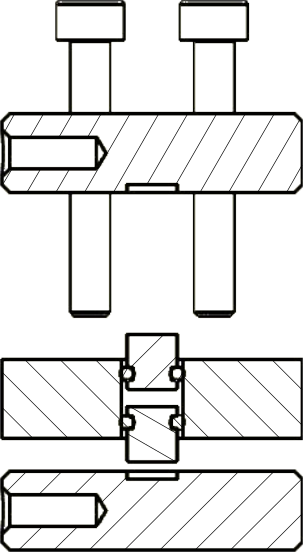
\includegraphics[width=0.2\textwidth]{celda2.png}
		}
	\label{fig:celda_de_pruebas_SC}
\end{figure}


\section{Resultados}
Los supercondensadores son sometidos a pruebas electroquímicas para estudiar su desempeño, estás pruebas incluyen: voltametría cíclica (CV), ciclos de carga y descarga a corriente constante, espectroscopía de impedancia electroquímica (EIS).
